\section{习题参考答案}
\subsection*{一、填空题}
\begin{enumerate}
    \item 如果导体不是闭合的,即使导体在磁场里做切割磁力线运动也不会产生感应电流,但在导体的两端产生\anl{感应电动势}.
    \item 在磁感强度为~$\vec{B}$~的均匀磁场中,以速率$v$垂直切割磁力线运动的一长度为$L$的金属杆,相当于一个电源,它的电动势~$\varepsilon$=\anl{$vBL$}.
    \begin{note}
        \textcolor{red}{$\varepsilon=\int_L (\vec{v}+\vec{B}\cdot \dd \vec{l}=\int_{0}^{L}vB\dd l = vBL)$}
    \end{note}
    \item 半径为$R$的圆形回路,放在均匀磁场中,回路平面与$\vec{B}$垂直,当回路半径以恒定的速率$\frac{\dd R}{\dd t}$收缩,刚开始时回路中的感应电动势大小$\varepsilon$=\anl{$2\pi RB\frac{\dd R}{\dd t}$}.
    \begin{note}
       \textcolor{red}{$\varPhi=\pi R^2 B$, $-\frac{\dd \varPhi }{\dd t}=-\frac{\dd (\pi R^2 B)}{\dd t}=-2\pi RB\frac{\dd R}{\dd t}$}
    \end{note}
    \item 动生电动势计算公式为~$\varepsilon$=\anl{$\int_L \vec{v}\times \vec{B}\cdot \dd \vec{l}$}.
    \item 如图~\ref{Fig:89}:长为$L$的金属杆$OA$,在方向竖直向上,磁感应强度大小为$B$的均匀磁场中,以匀角速度$\omega$绕$OO'$轴逆时针(从上往下看)方向转动,转动过程中$OA$与$OO'$轴的夹角始终保持$60^\circ$不变,则$OA$上的动生电动势为\anl{$\varepsilon=\frac{3}{8}B\omega L^2$}.
    \insertfig{0.25}{fig89}{Fig:89}
    \begin{note}
        \textcolor{red}{$\varepsilon_L(\vec{v}\times\vec{B})\cdot\dd \vec{l}=\int_0^L vB\mathrm{sin}\frac{\pi}{2}\mathrm{cos}\frac{\pi}{2}\dd l$=$\int_0^L(l\mathrm{sin}\frac{\pi}{3}\omega)B\mathrm{sin}\frac{\pi}{2}\mathrm{cos}\frac{\pi}{6}\dd l=\frac{3}{8}B\omega L^2$}
    \end{note}
    \item 半径为~$a$~的无限长密绕螺线管,单位长度上的匝数为$n$,通以交变电流$I=I_0\mathrm{cos}\omega t$,则围在管外的同轴圆形回路(半径为~$r$~)上的感生电动势大小$\varepsilon$=\anl{$\pi a^2 \mu n I_0 \omega \mathrm{sin}\omega t$}.
    \begin{note}
        \textcolor{red}{$\frac{\dd \varphi}{\dd t}=\frac{\dd(\mu n I \pi a^2)}{\dd t}=\pi a^2 \mu n I_0 \omega \mathrm{sin} \omega t$}
    \end{note}
    \item 金属杆$ABC$处于磁感强度$B=0.1 T$的匀强磁场中,磁场方向垂直纸面向里(如图所示~\ref{Fig:90})。已知$AB=BC=0.2 \mathrm{m}$,当金属杆在图中标明的速度方向运动时,测得$A,C$两点间的电势差是~$3.0V$,则可知$A,B$两点间的电势差$V_{ab}$=\anl{$2.0V$}.
    \insertfig{0.25}{fig90}{Fig:90}
    \item 对于一自感为$L$的线圈来说,当其通电流为$I$时,磁场的能量$W$=\anl{$\frac{1}{2}LI^2$}.
    \item 反映电磁场基本性质和规律的积分形式的麦克斯韦方程组为:
    \twoch{$\oint_S \vec{D}\cdot \dd \vec{S}=\sum\limits_{i=1}^n q_i$}{$\int_l \vec{E}\cdot \dd \vec{l}=-\frac{\dd \phi}{\dd t}$}{$\oint_S \vec{B}\cdot \dd \vec{S}=0$}{$\oint_l \vec{H}\cdot \vec{l}=\sum\limits_{i=1}^{n}I_I+\frac{\dd \phi_e}{\dd t}$}\par
    试判断:变化的磁场一定伴随有电场,这个结论是包含于或等效于上述第\underline{\makebox[2em]{2}} 个麦克斯韦方程式。磁感应线是无头无尾的,这个结论是包含于或等效于上述第\\
    \anl{3} 个麦克斯韦方程式。
    \item 麦克斯韦电磁场理论的两个基本假设为:(1)\underline{位移电流};  (2)\underline{有旋电场};
\end{enumerate}
\subsection*{二、选择题}
\begin{enumerate}
    \item 如下图~\ref{Fig:91}~两个导体回路平行,共轴相对放置,相距为$D$,若沿图中箭头所示的方向观察到大回路中突然建立了一个顺时针方向的电流时,小回路的感应电流方向和所受到的力的性质是~\anss{C}
    \twoch{顺时针方向,斥力 }{顺时针方向,吸力}{逆时针方向,斥力}{逆时针方向,吸力}
    \insertfig{0.25}{fig91}{Fig:91}
    \item 如图~\ref{Fig:92} 一闭合导体环,一半在匀强磁场中,另一半在磁场外,为了环中感生出顺时针方向的电流,则应~\anss{B}
    \twoch{使环沿~$y$~轴正向平动}{使环沿~$x$~轴正向平动}{环不动,增强磁场的磁感应强度}{使环沿~$x$~轴反向平动}
    \insertfig{0.25}{fig92}{Fig:92}
    \item 如图,长度为$l$的直导线$ab$在均匀磁场~$\vec{B}$~中以速度$\vec{v}$移动,直导线$ab$中的电动势为~\anss{D}
    \fourch{$Blv$}{$blv\mathrm{sin}\alpha$}{$Blv\mathrm{cos}\alpha$}{0}
    \begin{note}
        \textcolor{red}{没有切割磁力线}
    \end{note}
    \item 在下列描述中正确的是~\anss{B}
    \onech{感生电场和静电场一样,属于无旋场}{感生电场和静电场的共同点,就是对场中的电荷具有作用力}{因为感生电场对电荷具有类似于静电场对电荷的作用力,所以在感生电场中也可类似于静电场一样引入电势}{感生电场和静电场一样,是能脱离电荷而单独存在。}
    \item 感生电场是~\anss{A}
    \onech{由变化的磁场激发,是无源场}{由电荷激发,是有源场}{由电荷激发,是无源场}{由变化的磁场激发,是有源场}
    \item 两个相同的线圈,每个自感系数均为$L_0$,将它们顺向串联起来,并放得很近,使每个线圈所产生的磁通量全部穿过另一个线圈,则该系统的总自感系数为~\anss{D}
    \fourch{0}{$L_0/2$}{$2L_0$}{$4L_0$}
    \begin{note}
        \textcolor{red}{具体如下:}
        \begin{figure}[H]
            \centering
            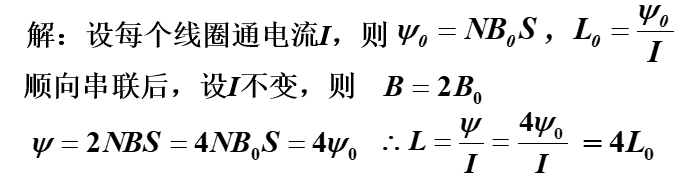
\includegraphics[width=0.55\textheight]{ans65}
        \end{figure}
    \end{note}
    \item 下列说法中唯一错误的说法是~\anss{D}
    \onech{涡旋电场是无源场}{涡旋电场的力线是闭合线}{涡旋电场在导体中形成持续电流}{涡旋电场的场强依赖于导体的存在}
    \item 两个相距不太远的平面圆线圈,以下哪种方法可使其互感系数近似为零~\anss{C}
    \twoch{两线圈的轴线互相平行放置}{两线圈并联}{两线圈的轴线互相垂直放置}{两线圈串联}
    \item 真空中一根无限长直细导线上通电流$I$,则距导线垂直距离为a的空间某点处的磁能密度为~\spaces
    \twoch{$\frac{1}{2}\mu_0(\frac{\mu_0 I}{2\pi a})^2$}{$\frac{1}{2\mu_0}(\frac{\mu_0 I}{2\pi a})^2$}{$\frac{1}{2}(\frac{2\pi a}{\mu_0I})^2$}{$\frac{1}{2\mu_0}(\frac{\mu_0 I}{2a})^2$}
\end{enumerate}
\subsection*{三、计算题}
\begin{enumerate}
    \item 如图~\ref{Fig:94}一面积为$1\mathrm{cm}^2$的小线圈在与其共面载电流为$I$的长直导线产生的磁场中,以速度$V$作匀速直线运动,方向与长直线导线垂直,已知$I=2A$,$V=3\mathrm{m/s}$,则当小线圈在图2位置时的电动势大小是多少?
    \insertfig{0.3}{fig94}{Fig:94}
    \begin{solution}
        如图:
        \begin{figure}[H]
            \centering
            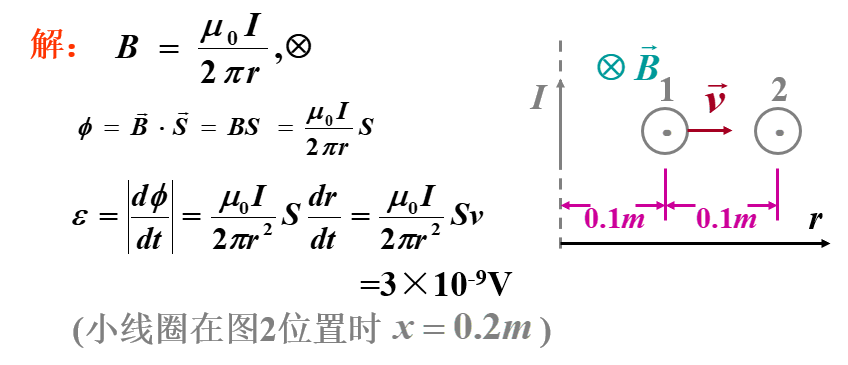
\includegraphics[width=0.55\textheight]{ans66}
        \end{figure}
    \end{solution}
    \item 如图所示~\ref{Fig:95},在两无限长载流导线组成的平面内,有一固定不动的矩形导体回路。两电流方向相反,若有电流~$I=I_0\mathrm{cos}\omega t$,(式中,$I_0$, $\omega$为大于0的常数)。求线圈中的感应电动势。
    \insertfig{0.2}{fig95}{Fig:95}
    \begin{solution}
        如图:
        \begin{figure}[H]
            \centering
            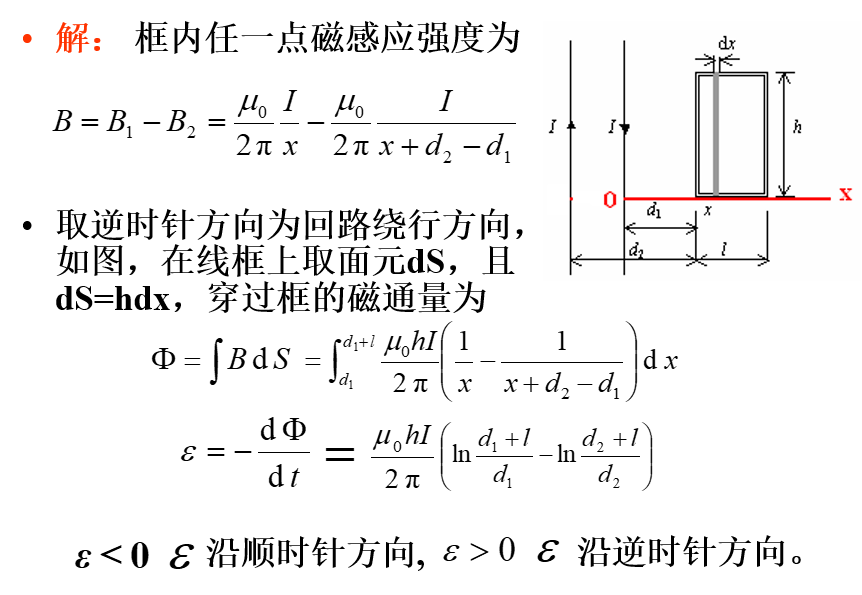
\includegraphics[width=0.55\textheight]{ans67}
        \end{figure}
    \end{solution}
    \item 一螺绕环横截面的半径为$a$,中心线的半径为$R$, $R>>a$,其上由表面为绝缘的导线均匀地密绕两个线圈,一个$N_1$匝,另一个$N_2$匝,试求:
    \begin{enumerate}[label=(\arabic*)]
        \item 两线圈的自感系数$L_1$和$L_2$.
        \item 两线圈的互感系数~$M$.
        \item $M$与$L_1$、$L_2$的关系.
    \end{enumerate}
    \begin{solution}
        如图:
        \begin{figure}[H]
            \centering
            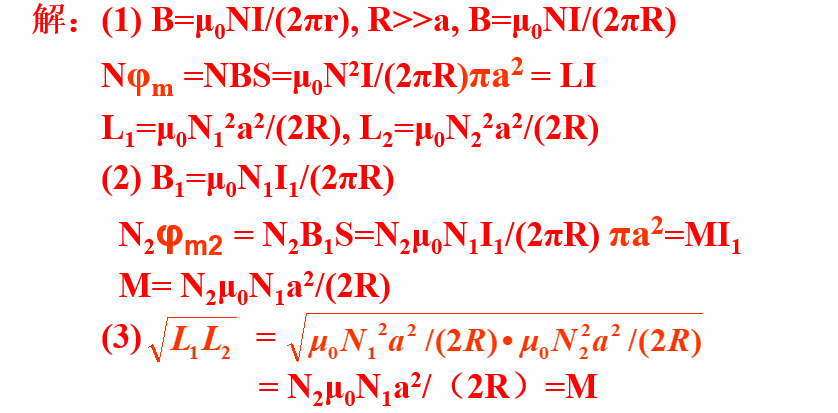
\includegraphics[width=0.55\textheight]{ans68}
        \end{figure}
    \end{solution}
\end{enumerate}